% -*-latex-*-

% Creation:    27-Nov-1995 Lutz Bauer (RWTH)
% Last Change: %G% , Lutz Bauer (RWTH)
% Release:     %R%
%
% -----------------------------------------

\newcommand{\bd}	{\begin{description}}
\newcommand{\ed}	{\end{description}}


\newcommand{\gadsize}	{0.9cm}
\newcommand{\gadsizep}	{1.1cm}

\chapter{The ConceptBase Usage Environment}
\label{cha:workbench}

This chapter describes the old user interface based on the
X window system. 

\section{ConceptBase Workbench}			\label{sec:workbench}

The {\em ConceptBase\/Workbench}  window is always present on the screen during a session. (see Figure \ref{fig:cbwb})

   	      \begin{figure}[htb]
              \centering
              \resizebox{13cm}{!}{\rotatebox{270}{\includegraphics{cbwb.eps}}}
              \caption{\label{fig:cbwb} The {\em ConceptBase\/Workbench}  main window.}
              \end{figure}

The numbers in Figure \ref{fig:cbwb} refer to the following areas in the {\em ConceptBase\/Workbench} 
 main window:
\begin{description}
\item[1.  Menubar.] The Menubar provides a set of functions, explained in Section \ref{sec:menubar}.
\item[2.  Smart Icon Panel.] The Smart Icons provide Editor--related functions like Cut, Copy, Paste, Tell, Untell, Ask, etc. See Section \ref{sec:icon_panel}.
\item[3.  Editor Field.] The Editor field allows easy editing of Telos syntax, described in Section  \ref{sec:editor}.
\item[3a. Editor Slider.] Scrolls the edited text.
\item[4.  Protocol Field.] Shows the   interaction protocol between the {\em ConceptBase\/Workbench}  and {\em ConceptBase}   Server. Please refer to Section \ref{sec:protocol} .
\item[4a. Protocol Slider.] Scrolls the protocol text.
\item[4b. Protocol bar.] Resizes the Protocol Field. Just click and drag bar to change size. 
\item[5.  Statusline.] Provides  status information such as connected state, success of the last transaction, etc. See Section \ref{sec:statusline}.
\end{description}

The following subsections explain the forementioned functional areas of the {\em ConceptBase\/Workbench}.

\subsection{Menubar} 			\label{sec:menubar}
The menubar consists of the following menu points:

\begin{description}
\item[Server]
   The Server menu contains all client server administration related functions as well as model and protocol related functions. It has the following submenus:
	\begin{description}
	\item[Connect CB Server ...]: Opens the registration window. It asks for the portnumber and the hostname of the desired server. If the button "Connect" is pressed {\em ConceptBase\/Workbench}  tries to connect the application with the given server. The success or failure of this function is displayed in the Statusline (see Section \ref{sec:statusline}). 
	\item[Disconnect CB Server]: Ends the connection between the Server and the {\em ConceptBase} {\em Workbench}. You don't {\em have} to disconnect from the server normally as the {\em ConceptBase\/Workbench}  disconnects automatically when it terminates. 
	\item[Model]:
	  	\begin{description}
	 		\item[Load model ...]: Selects a {\tt *.sml} file via a file--requesting dialogue and aks the server to load it as a model.
	 		\item[Save model ...]: Select a {\tt *.sml} file as destination to store the frames of the instances of a given object.
		  \end{description}
	\item[Protocol]:
		\begin{description}
			 \item[Load protocol ...]: Loads an ASCII file into the protocol.
			 \item[Save protocol ...]: Saves the protocol as an ASCII file.
		\end{description}
 	\item[Report clients ...]: Lists the current users of the  CBserver we are connected to. 
	\item[Stop server]: Stops the CBserver, which is connected with the {\em ConceptBase\/Workbench}.			
	\item[Quit]: Stops the {\em ConceptBase\/Workbench}  and disconnects the server if necessary.
	\end{description}

%\reversemarginpar

	\item[Edit] The Edit menu is divided into four different sections of submenus:
     \begin{description}
     \item[]
	The first group of Edit functions addresses the usual clipboard actions:
	\begin{list}{}{\setlength{\labelwidth}{\gadsizep} \labelsep0.8cm \listparindent0cm \itemindent0cm }
	\item[\mbox{\fbox{\resizebox{\gadsize}{!}{\includegraphics{cut.ps}}}}]
		{\bf Cut:} Allows you to copy the range of text, which can be marked by holding the left mouse-button while moving the mouse over the text, into a buffer for further use.
		Any marked text will be removed  from the Editor field after applying the Cut operation.
	\item[\mbox{\fbox{\resizebox{\gadsize}{!}{\includegraphics{copy.ps}}}}]
		{\bf Copy:} Does almost the same as Cut, only the marked range will remain inside the editor field.
	\item[\mbox{\fbox{\resizebox{\gadsize}{!}{\includegraphics{paste.ps}}}}]
		{\bf Paste:} Inserts the range of text, previously selected by Cut or Copy, at the position of the cursor  into the text of the editor.
		
	\end{list}
     \item[]
	The second group of Edit functions supports  server access:
	
	\begin{list}{}{\setlength{\labelwidth}{\gadsizep} \labelsep0.8cm \listparindent0cm \itemindent0cm }
	\item[\mbox{\fbox{\resizebox{\gadsize}{!}{\includegraphics{tell.ps}}}}]
		{\bf Tell:} The current text is communicated to the {\em ConceptBase} server, where an integration into the knowledge base is attempted. The success of this function is displayed in the Statusline (see Section \ref{sec:statusline})
		
	\item[\mbox{\fbox{\resizebox{\gadsize}{!}{\includegraphics{untell.ps}}}}]
		{\bf Untell:} The objects represented by the current text are `removed' from the knowledge base of the {\em ConceptBase} server and `entered' in the historical knowledge base.
		
	\item[\mbox{\fbox{\resizebox{\gadsize}{!}{\includegraphics{ask.ps}}}}] 
		{\bf Ask:} The current text is interpreted as a query, which is answered by the {\em ConceptBase} server; the answer will be displayed in a specific answer window.
		
	\end{list}
	The current text is either the actually selected text or {\em all} contents of the editor (if nothing is selected).
	All server interaction but browsing can be done with these three functions. The contents of the Telos editor  represents the frame(s) to {\bf Tell} or {\bf Untell} or the question to {\bf Ask}. Then you invoke the appropriate function and the result will be written to the Telos editor. In the case of Tell and Untell you could read the success from the state of the completion symbol in the lower left corner. If the protocol field is visible, you will see both the question and the answer as separated regions.
	If you wish to change the answer format, you should use the menu item {\bf Options/Ask answerformat}. For further help refer to the helptext of the options menu.

     \item[]
	The third group of Edit functions consists of loading frames to the editor, calling a query by name and renaming object labels.
	\begin{list}{}{\setlength{\labelwidth}{\gadsizep} \labelsep0.8cm \listparindent0cm \itemindent0cm }
	\item[  ] {\bf Call query:} Calls a query by its name from within the Telos editor. 

	\item[\mbox{\fbox{\resizebox{\gadsize}{!}{\includegraphics{load_frame.ps}}}}] 	{\bf Load frame:} Loads a given object in Telos frame representation into the  Editor field. In the Interaction--window you have to enter the name of the object to be loaded. You should use this function if you want to edit an existing object or to generate a similar one.
	
	\item[  ] {\bf Rename label:} Rename the Object--label of an {\tt Individual} object. {\bf Note!} Please do not rename the label of any SystemClass objects ! This may cause severe malfunction of the ConcepBase Server. Furthermore, the textual representation of Rules and Constraints is not affected by this function (i.e. the old Object--labels will not be replaced in the assertion text) -- though all Rules and Constraints will work with the new object labels.
	\end{list}

     \item[]	
	The last group of the Edit menu allows a textual search of editor and protocol fields. Furthermore you can access the protocol as a ringbuffer for the Telos editor. The concept of regions is explained in Section \ref{sec:protocol}.
	\begin{list}{}{\setlength{\labelwidth}{\gadsizep} \labelsep0.8cm \listparindent0cm \itemindent0cm }
		\item[{\bf Search}]: 
			Opens the search tool which provides a simple textual search in the editor window. The Search tool has the following fields:
				\begin{description}	
				\item[Search]: enter the pattern where to look for
				\item[Cancel]: leaves the search tool.
				\item[Help]: Displays a short help information
				\end{description}
			Remark: If you press the Return-Key, all found positions are marked. The number of  occurrences will be displayed in the statusline (see Section \ref{sec:statusline}).
			The scope of the search tool comprises the Telos-editor and the protocol field.
			Especially the search within a protocol can be  useful if you'd like to find any old information of the current session.
		\item[\mbox{\fbox{\resizebox{\gadsize}{!}{\includegraphics{new.ps}}}}]
			{\bf Clear Editor Buffer:} 
			Clears the buffer of the Telos editor.
		\item[\mbox{\fbox{\resizebox{\gadsize}{!}{\includegraphics{back.ps}}}}]
			{\bf Previous region:} Copies the previous region from the protocol to the Telos editor.
		\item[\mbox{\fbox{\resizebox{\gadsize}{!}{\includegraphics{next.ps}}}}]
			{\bf Next region:} Copies the next region from the protocol to the Telos editor.
	\end{list}
	
    \end{description}

\item[Browsing] This sub--menu calls different browsing tools :
\begin{description}
	\item[Display Instances]: You can choose a source class and the browser will display all its instances. You can iterate this process and finally copy the desired instance as Telos-frame to the Telos-editor. This tool is explained in Section \ref{sec:displayinstances}.
	\item[Display Queries]: Lists all  queries known to the {\em ConceptBase}  server. You can copy a selected query as Telos-frame to the Telos-editor. Alternatively you can pick it to open the parameter mask of the query, from which the server could be asked with the specified parameters. See Section \ref{sec:displayqueries} for more information.
	\item[Browse Graphical]: Starts the external {\em Graphbrowser}. Refer to Section \ref{sec:graphbrowser} for full information on the {\em Graphbrowser}  Utility.

	%\item[Browse Hierarchical]: Starts the external hierarchical browser
\end{description}

\item[Options]
The  Options sub--menu supports the adjustment of different options:
\begin{list}{}{\setlength{\labelwidth}{\gadsizep} \labelsep0.8cm \listparindent0cm \itemindent0cm }
	%\item[Paths ...]: Opens a dialog to reset the path to the external browsers. Normally, you
	% shouldn't need to adjust the path.
	\item[  ] {\bf Overwrite TelosEditor:} If the Overwrite--item is checked  the Telos editor will be cleared before a new server operation. Those transactions  are a double--click in the protocol to copy the block or the activation of a button "Telos Editor" within the "display instance" or "display queries". If this item is not selected the new texts will appended into the Telos editor and the buffer becomes increases.
	\item[\mbox{\fbox{\resizebox{\gadsize}{!}{\includegraphics{time.ps}}}}]
	{\bf Rollbacktime ...:} Starts a dialog for setting a rollbacktime that will be used for accessing the server. Please keep in mind that ConceptBase runs in Greenwich Mean Time(GMT), therefore you have to adjust the Rollbacktime to GMT. Note: this  rollbacktime is not valid for the {\em Graphbrowser}  Utility (see Section \ref{sec:graphbrowser}). 
	\item[  ] {\bf Ask answerformat:} Choose between Telos, FRAGMENT and LABEL as the answerformat of all answers from the server to any  queries.
	\item[  ] {\bf Default connection ...:} If the {\em ConceptBase\/Workbench}  is frequently used  while the CBserver is  running on the same host with the same portnumber, then you could automate the connection by activating this option.
	\item[  ] {\bf Display instances origin ...:} Determines the default origin for the display instances dialog.
	\item[{\bf Graphical browser  ...:}]  This submenu provides functions to adjust graphbrowser specific  properties. 
		  	\begin{description}
	 		\item[Origin ...]: Determines the default origin for the graphical browser startup dialog.
	 		\item[Palette ...]: Determines wether the GraphBrowser should run with a Color or Monochrome Palette.
		  \end{description}
	% \item[Hierarchical browser ...]: Sets the default values for the hierchical browser startup dialog.
	\item[{\bf Save options:}] Saves altered options to the file "{\tt .CBworkbench.usr}" in the HOME-directory of the user.


\end{list}

\item[Help] The Helpmenu provides most of the information which was presented in this section on all available menus, the Editor field, the Protocol field and the status line. All dialogue Windows as well as the Browsing tools contain their own Help buttons too.

\end{description}

\normalmarginpar

\subsection{Smart Icon Panel}			\label{sec:icon_panel}
	      \begin{figure}[htb]
              \centering
              \resizebox{\textwidth}{!}{\includegraphics{gadgets.eps}}
              \caption{\label{fig:gadgets} The {\em ConceptBase\/Workbench}  Smart Icon Panel.}
              \end{figure}

The Smart Icon Panel provides  quick access to the most frequently used functions from  the {\bf Edit Menu} (for  a description, please refer to Section \ref{sec:menubar}).  Figure \ref{fig:gadgets} shows the Icon-Representation of these edit functions.  To select a function, just click the corresponding icon using the left mouse--button.  Note: All Editor--functions can be called via  a so--called {\em Short-cut} (in brackets) for quick \& easy keyboard access (See Fig. \ref{fig:shortcuts}).  \\

\begin{figure}[htb]
\centering
\begin{tabular}{|l|l|}
\hline
Command			&	Shortcut  	\\ 	     
\hline
{\bf  Cut}		&	(Ctrl + W)	\\
{\bf  Copy }		&	(Meta + W)	\\
{\bf  Paste }		&	(Ctrl + Y)	\\
{\bf  Tell }		&	(Alt + E + T)	\\
{\bf  Untell }		&	(Alt + E + U)		\\
{\bf  Ask }		&	(Alt + E + A)		\\
{\bf  Load Frame }	&	(Alt + E + L)		\\
{\bf  Clear Editor buffer }	&		(Alt + E + C)	\\
{\bf  Previous region } &	 (Alt + U)	\\
{\bf  Next region }	&	(Alt + D)	\\
{\bf  Set Rollbacktime}	& 	(Alt + O + R)		\\
\hline
\end{tabular}
 \caption{\label{fig:shortcuts} Short-cuts of the most frequently used Editor-functions}
\end{figure}

\subsection{Telos Editor Field} 			\label{sec:editor}
The {\em Telos Editor} is used to display, modify and create Telos objects. The Editor field (see Figure \ref{fig:cbwb}) acts like a normal text Editor: you can move the cursor using the Arrow-Keys, locate the cursor by mouse--clicking, mark blocks by keeping the left mouse--button pressed \& moving the mouse. Normal Editor functions like Cut, Copy \& Paste are called from either within the Menubar (see Section \ref{sec:menubar}), the Smart Icon Panel or by a Short--cut keystroke (see Section \ref{sec:icon_panel}). As a special feature, double clicking on a Telos--Object name inside the Editor field, loads the corresponding object frame into the Editor field. \\
As a default setting, every new input is appended to the current content of the Editor when you either load a frame or double--click a region in the Protocol field (see Section \ref{sec:protocol}). If you'd like the editor field to be cleared before the new content is displayed, use the {\em Overwrite Telos Editor } Option from the Options menu (see Section \ref{sec:menubar}).



\subsection{Protocol Field}				\label{sec:protocol}
The Protocol field provides a logbook of the dialogues held between the {\em ConceptBase\/Workbench}  and different {\em ConceptBase Servers}. All  performed operations are echoed by operation name (either Load Frame, Tell, Untell or Ask) and the Telos Frames involved in the operation. \\

The protocol ist divided into so--called {\bf regions}. A region is marked by a background colour, either white (normal message) or black (Error message). Regions always contain feedback information from the {\em ConceptBase}  server on the previous operation.
Every access like {\bf Tell}, {\bf Untell}, {\bf Ask} or {\bf Load Frame} has its own region--representation. 
For example a Query adds two new regions to the protocol. The first  region for {\bf Ask:} contains the query, and the second  region for {\bf Answer:} shows the answer if it was succesful, otherwise and {\bf Error:} region occurs with the appropriate message.
Additionally, you can perform different actions on a selected region (double--click to select a region). Each action is called from a pop--up menu, invoked by pressing the right mouse--button inside the selected region. The following actions exist:
\begin{description} 
\item[Copy To Telos Editor] Copies the selected region to the Telos Editor field (not available for Error regions). Note: you can also call this function by double--clicking the region in the protocol field. 
\item[New View Window] Copies the selected region into a newly created  "`buffer"' window. This can be used to keep different regions in view at the same time. The View window provides normal {\bf Cut} and {\bf Paste} functions. You can also copy the content of the View window into the Editor field by clicking the provided {\bf Copy}--button of the view window. This allows for instance easy switching between different Query frames for repeated asks.
\item[Delete Region] Deletes the selected region from the protocol field.
\item[Tell Region] Performs a Tell operation on the selected region content.
\item[Untell Region] Performs an Untell operation on the selected region content.
\item[Ask Region] Performs an Ask operation on the selected region content.
\end{description}

You can resize the Protocol field by clicking and dragging the Protocol bar. 
The protocol can be loaded and saved as an ASCII file in the menubar (protocol submenu) -- but all region structures are lost.



\subsection{Statusline}				\label{sec:statusline}
	      \begin{figure}[htb]
              \centering
              \resizebox{\textwidth}{!}{\includegraphics{statusline.eps}}
              \caption{\label{fig:statusline} The {\em ConceptBase\/Workbench}  Statusline.}
              \end{figure}

The statusline displays certain status information about the current session at the bottom of the {\em ConceptBase\/Workbench}  Window:
From left to right you will find (according to Fig. \ref{fig:statusline}):
\begin{enumerate}
\item A checkbox which is green--coloured if the last server access was ok. Otherwise, in the case of error occurence, the checkbox will become red. The advantage of the checkbox is that you can see the difference, even if you are using a monochrome display.
\item (connected/disconnected): Displays the state of  connection to the server.
\item rollback:$\langle $time$\rangle $ Shows the currently valid rollbacktime. The rollbacktime can be altered either from the Smarticon Panel (see Section \ref{sec:icon_panel}) or the Menubar (see Section \ref{sec:menubar}).
\item A field for the search tool to display the number of found positions of a search.
%\item t:$\langle $time$\rangle $ Exposes the time of the last server access.
%\item T:$\langle $timesum$\rangle $ Exposes the sum of accesses  during the session.
\end{enumerate}
%Note: That the last two informations are just of statistical nature.



\section{Browsing Utilities}

The {\em ConceptBase\/Workbench}  provides three different browsing facilities: the {\bf Display Instances} tool, the {\bf Display Queries} tool and the {\bf {\em Graphbrowser}}. 

\subsection{Display Instances}				\label{sec:displayinstances}
The Display Instances facility is used to display all instances of a given object.  Direct Instances are computed as well as inherited ones. The Display Instances tool is called from the {\em ConceptBase\/Workbench}  menubar (see Section \ref{sec:menubar}). 

The Display Instances window (see Figure \ref{fig:sess_display}) has the following features:

	 

\begin{description}
\item[Class String Field] Enter the wished origin of the  instances  to be displayed.
\item[First listbox] contains the found instances of the class
\item[History listbox] contains previous origins. 
\item[Display Instances Button] Takes the selected item as new origin to display its instances in the first list box.
\item[Telos Editor Button] Copies the frame of the selected object into the Telos-editor field of the {\em ConceptBase\/Workbench}.
\item[Cancel Button] Leaves the Display Instances tool.
\item[Help Button] Shows a help text.
\end{description}
	
If an item of the listboxes is selected by the $\langle $return--key$\rangle $ or $\langle $double--click$\rangle $
then a "`Display Instances"' operation is performed with the selected object as origin.



\subsection{Display Queries}				\label{sec:displayqueries}

Display Queries supports  asking queries with an automatic dialogue to fill the required parameters of the query.
  
 \begin{figure}[htb]
              \centering
              \resizebox{7cm}{!}{\rotatebox{270}{\includegraphics{queries.eps}}}
              \caption{\label{fig:display_q} The {\em Display Queries} Window.}
              \end{figure}     

Figure \ref{fig:display_q} shows the features of the Display Queries tool:

\begin{description}
\item[Listbox] Contains all Queries that are known to the server. To pick an item by $\langle $return--key$\rangle $ or $\langle $double--click$\rangle $ has the same effect as the button {\bf Ask}.
\item[Ask Button] Opens a  dialogue to determine the parameters of the query (see Figure \ref{fig:ask_parm}). The Ask Parameter dialogue requests all necessary parameters (if there are any) and substitutes them in the query. You can choose if you'd like instances or specialisations of your parameter in the appropriate options menu next to the corresponding parameter string field.
  Figure  \ref{fig:ask_parm} demonstrates the call of the query {\tt exists} which requires one {\tt objname} parameter.
\item[Telos Editor Button] Copies the frame of the selected object to the Telos-editor field of the {\em ConceptBase\/Workbench}.
\item[Cancel Button] Leaves the Display Queries tool.
\item[Help Button] Shows a help text.
\end{description}

  
\begin{figure}[htb]
              \centering
              \resizebox{7cm}{!}{\rotatebox{270}{\includegraphics{queries_par.eps}}}
              \caption{\label{fig:ask_parm} The Ask Parameter Dialogue.}
              \end{figure}



\subsection{GraphBrowser}					\label{sec:graphbrowser}

The {\em Graphbrowser}  Utility is invoked from the {\em ConceptBase\/Workbench}  menu item {\bf Browsing} submenu {\bf Browse Graphical}.
The {\em Graphbrowser}  requires  an object name and then draws the corresponding object as an initial node of a directed acyclic graph (DAG). After selecting the {\bf Browse Graphical} menu item, {\em ConceptBase\/Workbench}  requests the required object name parameter. \\

Note: the rollbacktime of the {\em ConceptBase\/Workbench}  is not valid inside the {\em Graphbrowser}, instead 
the value 'Now' is used as default. \\

After the {\em Graphbrowser}  shows up, you can select every displayed object by clicking the left mouse button. A selected object can be moved by dragging the object while keeping the left mouse button pressed. Note, that selecting and moving objects is also available for nodes and links. The following menu buttons are provided in the {\rm Graphbrowser} tool:

\begin{description}
\item[Erase Node] - deletes the selected object (node or link) from the display \footnote{Erasing an item from the {\em Graphbrowser} display has no impact on the Knowledge Base.}.
\item[Any] - displays all objects connected to the selected object by a link corresponding to a user-defined specification of orientation and label.
\item[Show Attributes] -  displays all  direct attributes (no inherited ones !);
\item[Show Instances] - displays all  direct instances (no derivable ones); not available if the selected object is a link;
\item[Show Classes] - displays all classes the selected object is an instance of; not available if the selected object is a link;
\item[Show Subclasses] - displays one level of subclasses (i.e. subclasses of a subclass of the selected node are not displayed); not available if the selected object is a link;
\item[Show Superclasses] - displays one level of superclasses (i.e. superclasses of a superclass of the selected node are not displayed); not available if the selected object is a link;
\item[Save Layout] Saves the current layout of the {\em Graphbrowser}  window to a specified file

\item[Load Layout] Loads a layout from file and arranges the graphical 
situation as specified in the file. Note: This function {\em only} 
succeeds, if {\em all} Objects specified in the layout file are still 
present in the current application.

\item[Help] -  Displays a Info text explaining the {\em Graphbrowser}'s facilities;
\item[Quit] - terminates the {\em Graphbrowser}.
\end{description}


An additional button is provided for invoking another {\em Graphbrowser}  with the selected object. If no object is selected, there is an additional option {\bf Add Node}. On selection of {\bf Add Node}, a new object with no connection to the existing graph is introduced at the position of the last left mouse click.


The style in which nodes or links are displayed in the {\em Graphbrowser}'s window, is 
modeled within the knowledge base by so--called {\em Graphical Types}, which belong to a certain palette. 
Using these types, you can totally customize the appearance of the 
{\em Graphbrowser} \ (e.g. you can specify your own Icon--shapes, Fontstyles, etc.). 
Please refer to Appendix \ref{cha:graph-typen} for an extensional 
description of this facility.

If you'd like to use a different palette, you may use the {\bf Graphbrowser...} menupoint in the {\em ConceptBase\/Workbench}\ {\bf Options} menu.


\section{An Example Session with ConceptBase}			\label{sec:session}


In this section we demonstrate the usage of the {\em ConceptBase\/Workbench}, by involving an example model. It consists of a few classes 
including {\tt Employee, Department, Manager}. The class {\tt 
Employee} has the attributes {\tt name, salary, dept, and boss}. In 
order to create an instance of {\tt Employee} one may specify the 
attributes {\tt salary, name,  and dept}. The attribute {\tt boss} 
will be computed by the system using the {\tt bossrule}. There is also a 
constraint which must be satisfied by all instances of the class {\tt 
Employee} which specifies that no employee may earn more money than its 
boss. The Telos notation for this model is given in Appendix 
\ref{sec:employee-model}.


\subsection{Starting ConceptBase}


To start a {\em ConceptBase} session, we use two terminal windows, one for the {\em ConceptBase} 
server and one for the usage environment. We start the {\em ConceptBase} server 
by typing the command {\tt CBserver -p 4200 -d test}  in a terminal 
window of, let us say machine alpha. Then we start the usage environment with 
the command {\tt CBjavaInterface} in the other window. 



\subsection{Connecting the Usage Environment to the ConceptBase Server}


\begin{figure}[htb]
              \centering
              \resizebox{5cm}{!}{\rotatebox{270}{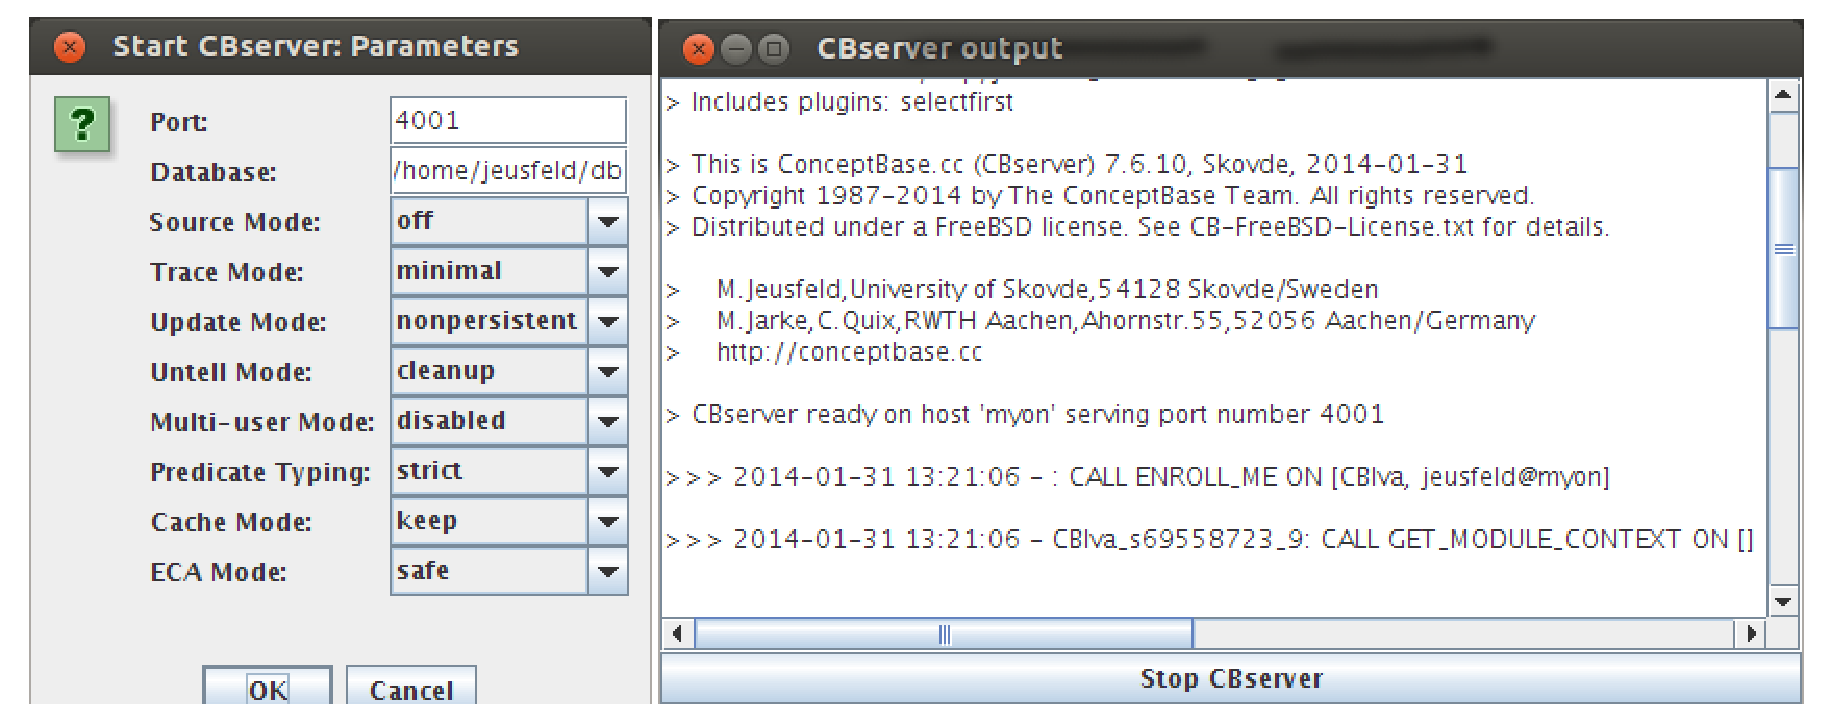
\includegraphics{startserver.eps}}}
              \caption{\label{fig:startserver} The Start Server Dialogue.}
              \end{figure}


Next we establish a connection between the {\em ConceptBase}  server and the usage 
environment. This is done by choosing the opition {\bf Connect CB 
Server} from the Server menu of the {\em ConceptBase\/Workbench}  menubar. An interaction window 
appears (see Figure \ref{fig:startserver}) querying for the host name 
and the port number of the server (i.e. the number we have specified within 
the command {\tt CBserver -p 4200 -d test}).  To connect the 
{\em ConceptBase\/Workbench}  directly to the {\em ConceptBase}--server, you can use the  auto--connect option (see the 
description of a default connection from the Options submenu in Section 
\ref{sec:menubar}).

    	\


\subsection{Loading Objects from external Files}


The objects manipulated by {\em ConceptBase} are persistently stored in a 
collection of external files, which reside in a directory called {\bf 
application} or {\bf database}. The actual directory name of the 
application is supplied as the -d parameter of the command {\tt 
CBserver}.


The -u parameter of the {\tt CBserver} specifies wether updates are made 
persistent or are just kept in system memory temporarily. Use {\tt -u 
persistent} for a update persistence or {\tt -u nonpersistent} for a 
non persistent update mode.


The application can  be modified interactively using the editor commands 
TELL/UNTELL. If {\tt -u persistent} is set, all activities like creating 
new objects or modifying existing objects are stored simultanously to the 
memory--resident KB and to the specified application files so that 
persistence of interactive updates is guaranteed. This is the usual way of 
extending an application. If the UpdateMode is set to {\tt 
nonpersistent} all interactive updates are not stored in the file system, but kept in system memory until the server run is stopped. \\


Another way of extending applications is to load Telos objects (expressed 
in frame syntax) stored in Unix files with the extension  *.sml. Call the menu 
item {\bf Load Model} from the {\bf Model} sub--menu of the {\bf Server--Menu} to include these objects 
into the {\em ConceptBase}  \ Knowledge base. In our example the application (directory) 
Employee was built interactively and can be found together with files 
containing the frames constituting the example in the directory


\begin{center}	{\em CB\_HOME}{\tt /examples/QUERIES} 
\end{center}


where you have to replace {\em CB\_HOME} with the {\em ConceptBase}  installation directory.  The 
following files contain the objects of the Employee example expressed in 
frame syntax:  {\tt Employee\-\_Classes.sml, Employee\-\_Instances.sml, 
 Employee\-\_Queries.sml}.  An alternative to interactively building an 
application is to start the server with an empty application ({\tt -d
}$\langle ${\tt newfile}$\rangle $) and  then add the objects in these files 
by using {\bf Load Model}. Note, that the *.sml extension may be omitted.
 During the load operation of external models, {\em ConceptBase}    
checks for syntactical and semantical correctness and reports all errors to 
the Protocol field as is done when updating the KB interactively using the 
editor. This protocol field collects errors reported since the beginning of 
the session. \



\subsection{Displaying Objects }


To display all instances of an object, e.g. the class {\tt Employee}, we invoke 
the Display Instance facility  by 
selecting the item {\bf Display Instances} from the menubar. In the 
interaction window we specify {\tt Employee} as object name. The 
instances of the class {\tt Employee} are then displayed (see Figure \ref{fig:sess_display}).


\begin{figure}[htb]
              \centering
             \resizebox{7cm}{!}{\rotatebox{270}{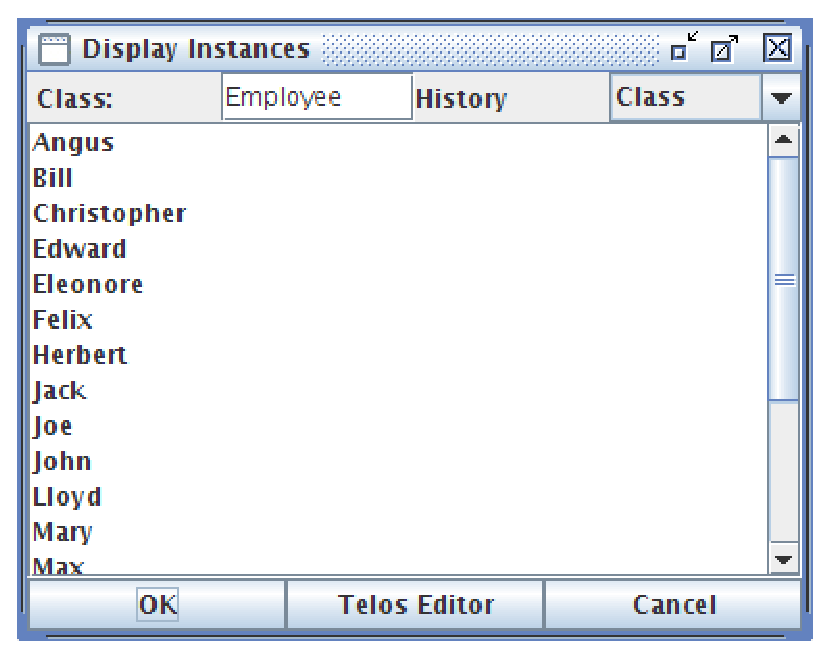
\includegraphics{session_display.eps}}}
              \caption{\label{fig:sess_display} Display of {\tt Employee} instances.}
\end{figure}

After selecting a displayed instance we can load the frame representation 
of an instance to the Telos Editor or display further instances. See Section \ref{sec:displayinstances} for an overview on the Display Instances facility.



\subsection{Browsing Objects}

For browsing through a loaded application in the KB we use the {\em GraphBrowser} \ Utility. 

The {\em GraphBrowser} (described in section \ref{sec:graphbrowser}) allows you display arbitrary objects from the current application. We display the object {\tt Employee} by choosing the {\bf Browse Graphical} function from the menubar and defining {\tt Employee} as the object to be browsed in the dialogue window provided.
After the {\em GraphBrowser} window shows up, we select the {\tt Employee} object and choose the {\bf Show Subclasses} option from the {\em GraphBrowser} menu. 
The displayed graph is now expanded (figure \ref{fig:graph_empl}). Notice, that the 
selected object, the node {\tt Employee}, is marked with small rectangles at each 
corner.


\begin{figure}[htb]
              \centering
             \resizebox{10cm}{!}{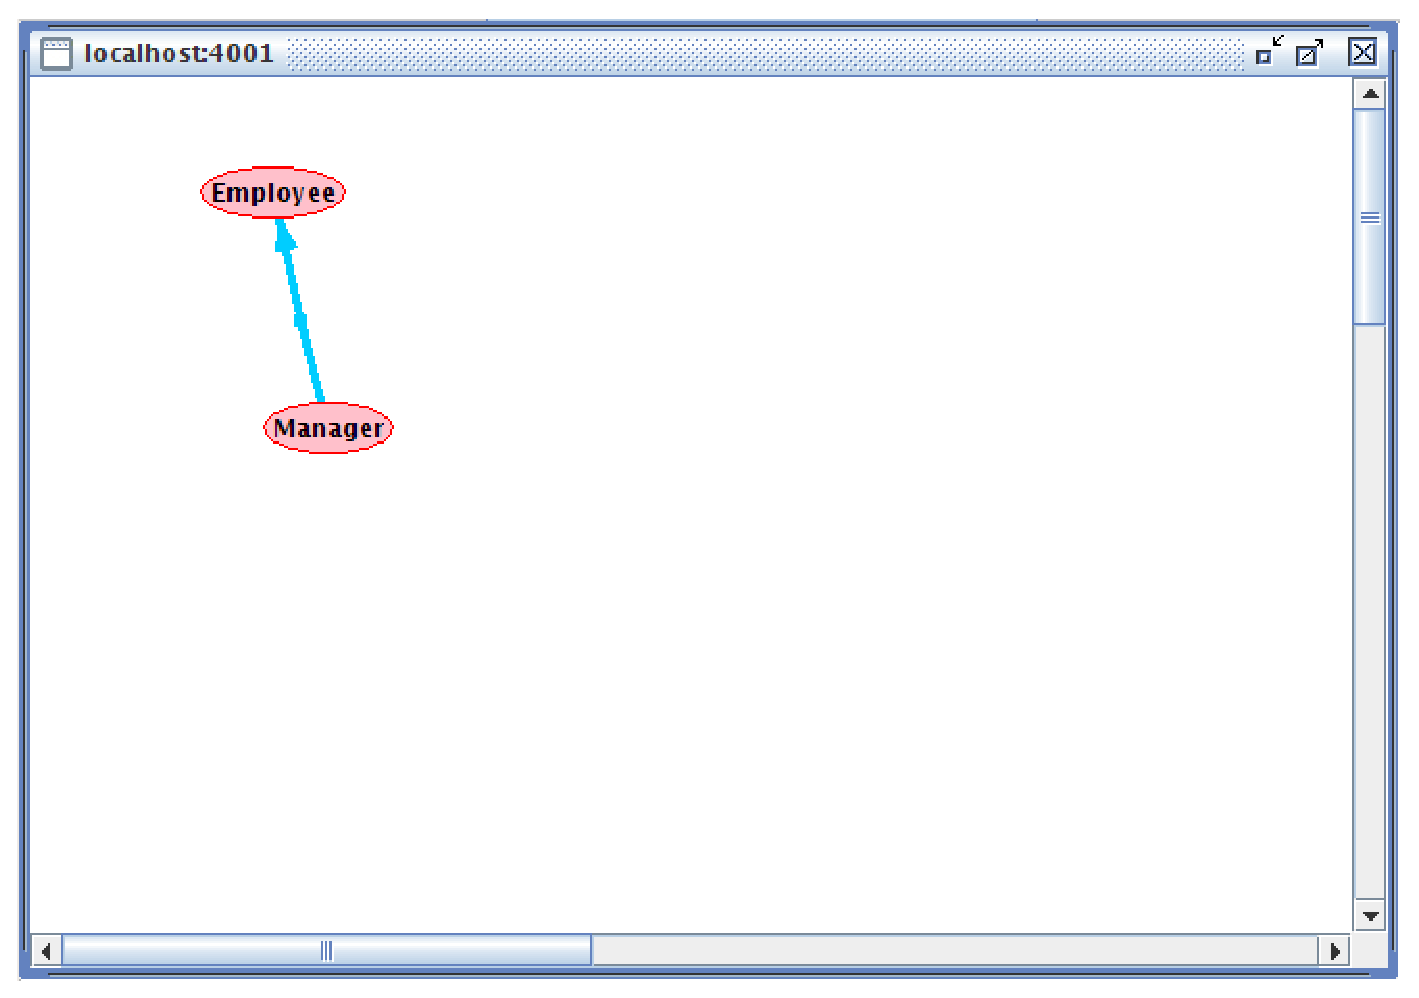
\includegraphics{graph_empl.eps}}
              \caption{\label{fig:graph_empl} The resulting graph after expanding the node {\tt Employee} with subclasses.}
\end{figure}



Now we expand the node {\tt Manager}, a subclass of {\tt Employee}, by choosing the 
{\em GraphBrowser} menu item {\bf Show Instances}. The resulting graph is shown in figure \ref{fig:graph_man}.

\begin{figure}[htb]
              \centering
             \resizebox{\textwidth}{!}{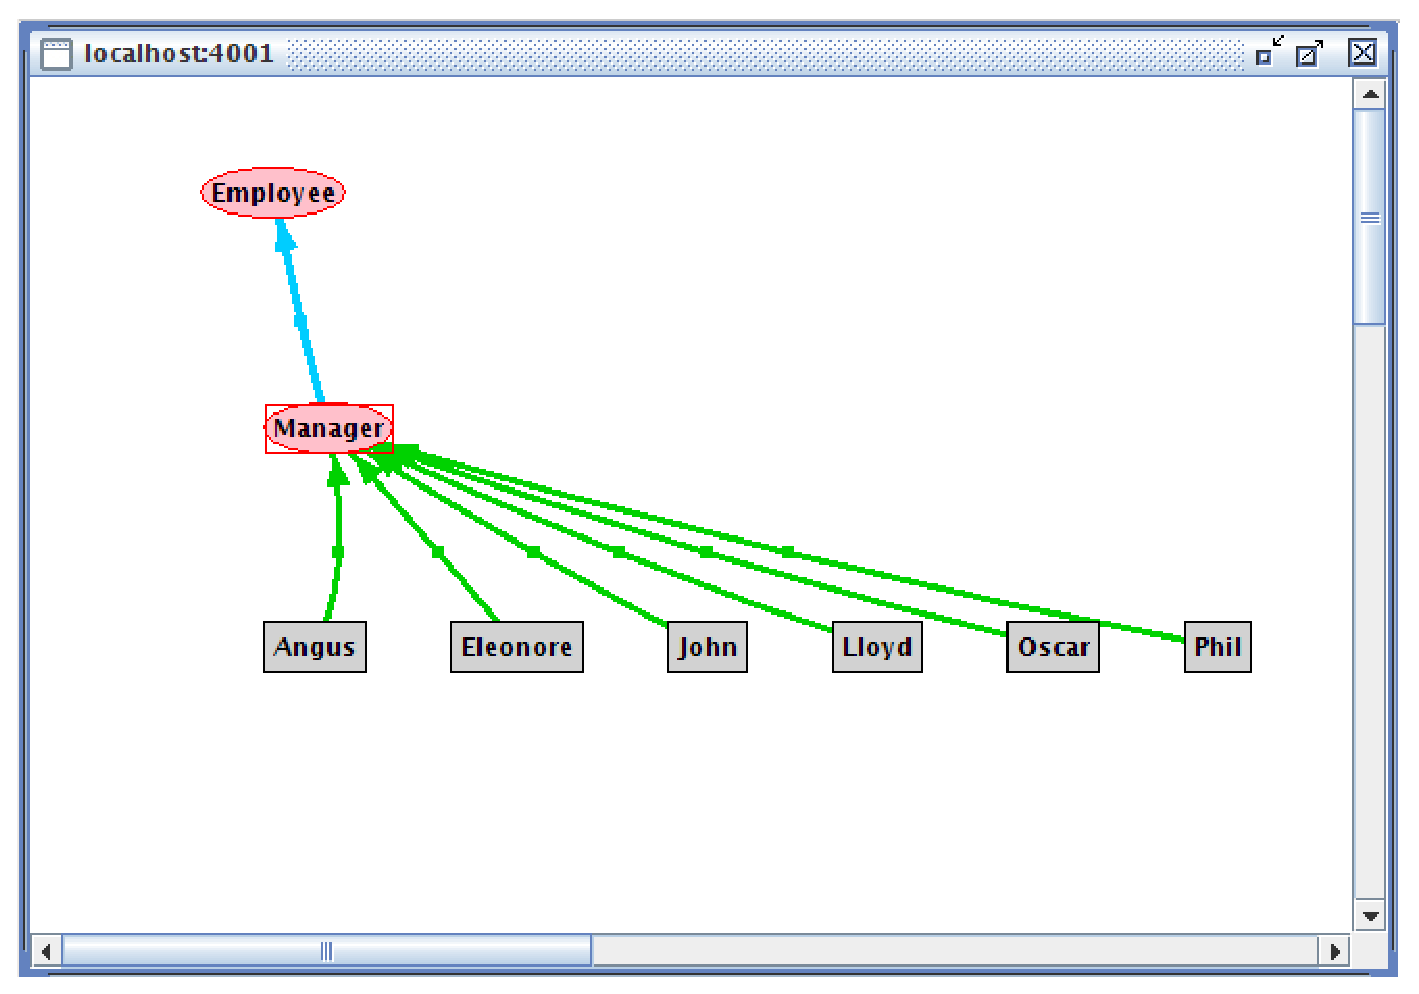
\includegraphics{graph_man.eps}}
              \caption{\label{fig:graph_man} The resulting graph after expanding with the instances of {\tt Manager}.}
\end{figure}



Now the selected object is the node {\tt Manager}. The instances of {\tt Manager} are 
shown as grey rectangles, because they are also instances of the system class 
{\tt Token}. The nodes {\tt Manager, Salesman, Employee} etc. are shown as ovals, 
since these nodes are instances of the system class {\tt SimpleClass} (see 
 for a full description of  graphical 
object semantics: Appendix \ref{cha:graph-typen}).


One can move nodes and links by selecting a node or a link and then holding 
down the left mouse button while moving the cursor to a different 
position. When the button is released the selected object will be located 
at the current position and the related links are redisplayed.



We select the node {\tt Employee} again and choose the menu item {\bf Any}. An 
interaction window appears querying for the orientation ({\tt coming\-\_out\-\_of, 
going\_into}, or simply {\tt c} and {\tt g}) and the label to be considered for the 
expansion of the displayed graph. We specify {\tt c} as orientation and 
`{\tt *instanceof}' as label, to see all the classes, where {\tt Employee} is an 
instance of. 
%The resulting graph gives an overview of the position of the 
% class {\tt Employee} in our knowledge base.
 To see the attributes of the class 
{\tt Employee} we choose the menu option {\bf Show Attributes} (the node {\tt Employee} 
should still be selected). Figure \ref{fig:graph_super} shows the resulting graph. Some of 
the nodes have been manually moved to present a clearer picture. \


\begin{figure}[htb]
              \centering
             \resizebox{\textwidth}{!}{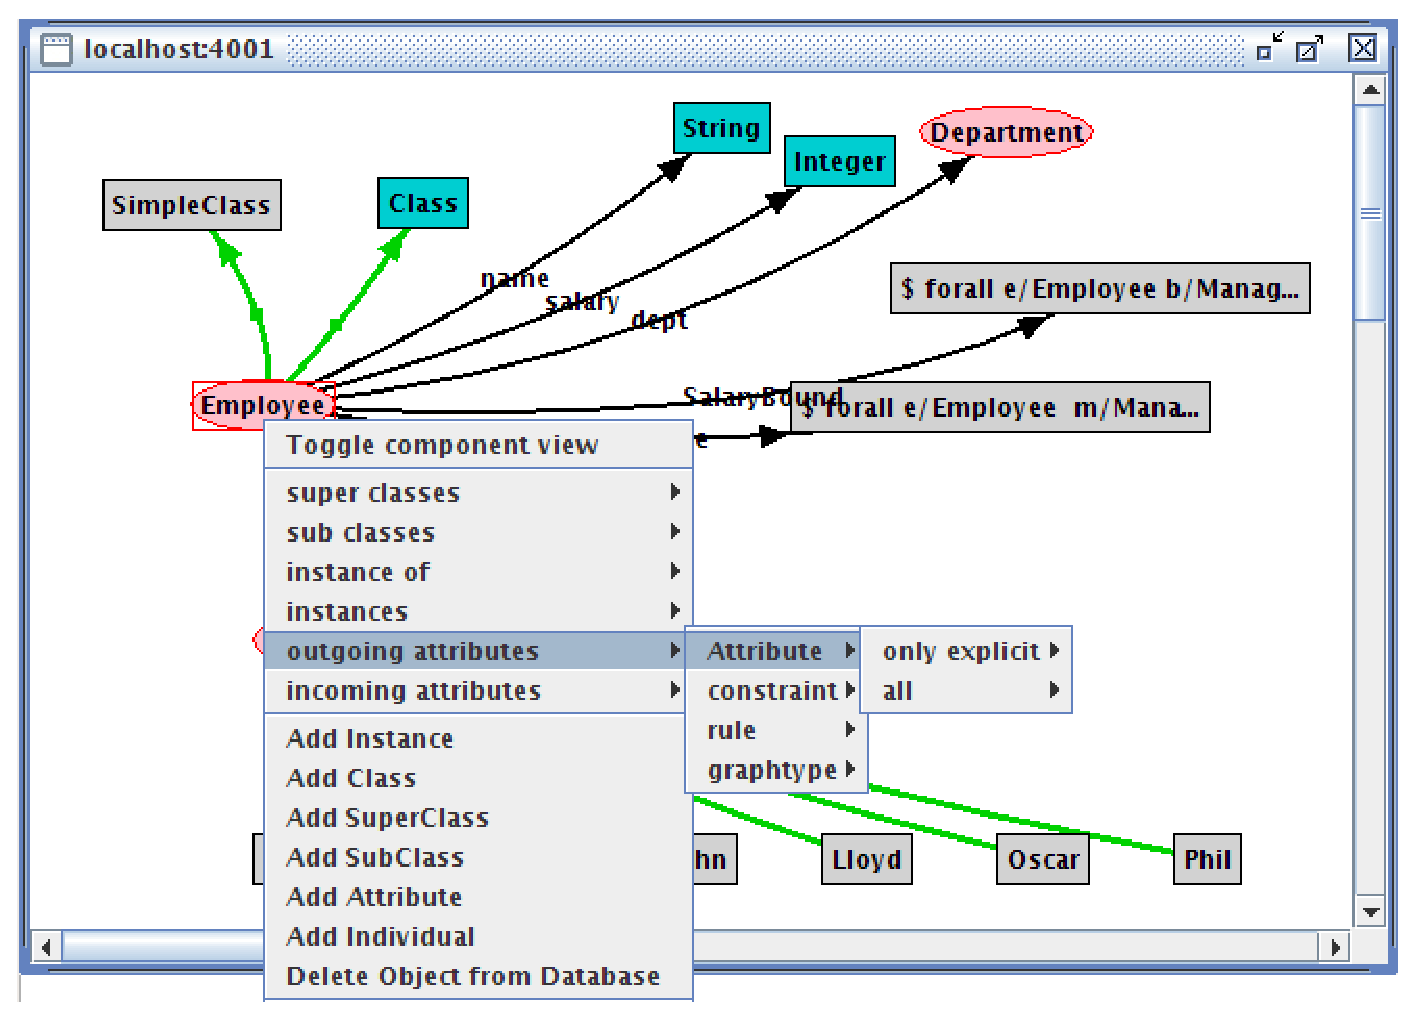
\includegraphics{graph_super.eps}}
              \caption{\label{fig:graph_super} The graph after expanding it with the superclasses and the attributes of the class {\tt Employee}. }
\end{figure}




\subsection{Editing Telos Objects}


Before we're able to edit a Telos object, we have to load it's frame representation in to the Telos Editor field first.
For loading a Telos object to the Editor field, we choose the {\bf Telos Editor} Button from either the Display Queries oder Display Instances Browsing facilities or the {Load Frame} button from the
{\em ConceptBase\/Workbench}\ window (see Figure \ref{fig:Telos_ed}).


\begin{figure}[htb]
              \centering
             \resizebox{13cm}{!}{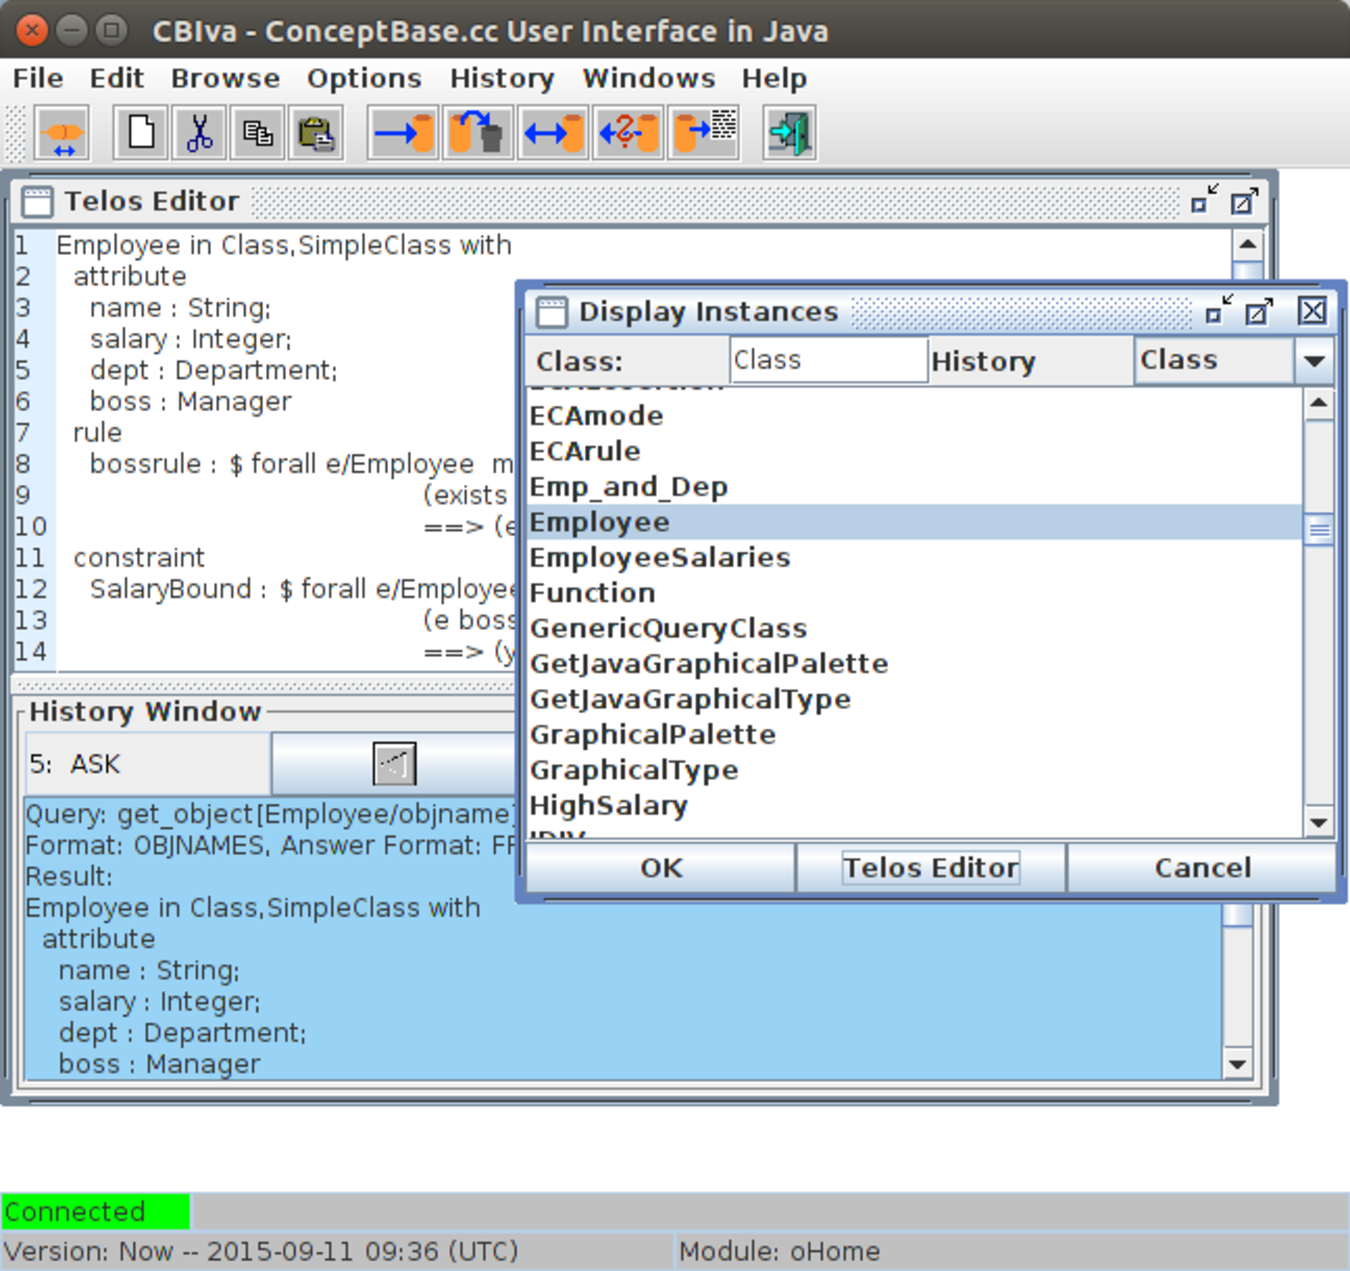
\includegraphics{telos_ed.eps}}
              \caption{\label{fig:Telos_ed}  The TelosEditor Field with the object {\tt Employee}.}
\end{figure}



Now we add an additional attribute, e.g. {\tt education}, to the class {\tt Employee} 
(for the description of the Telos syntax see Appendix \ref{cha:syntax}). The added 
statement is highlighted in figure \ref{fig:Telos_ed_error}. To demonstrate error reports from the {\em ConceptBase\/Workbench}\ and how to correct them, we have made mistakes in the syntax 
notation of the added attribute.


By clicking the left mouse button on the {\bf Tell} icon (see Section \ref{sec:icon_panel}) the content of the 
editor is told to the {\em ConceptBase}  server. Syntactical and semantical 
correctness is checked and the detected errors are reported to the Protocol field. The report resulting from our mistakes by specifiing the syntax of 
the new attribute is also shown in figure \ref{fig:Telos_ed_error}.


We correct the error by changing the added line from {\tt education : Strung;} to 
{\tt education   :  String;} and choose the {\bf Tell} symbol again. This time, 
since there are no further mistakes, the additional attribute is added to 
the class {\tt Employee}.


Now we can choose again the item {\bf Show Attributes} from the panel of the {\em GraphBrowser} \ window\footnote{The node Employee should still be selected.}
The additional attribute {\tt education}, added by using the Editor field, should be then displayed.

\begin{figure}[htb]
              \centering
             \resizebox{13cm}{!}{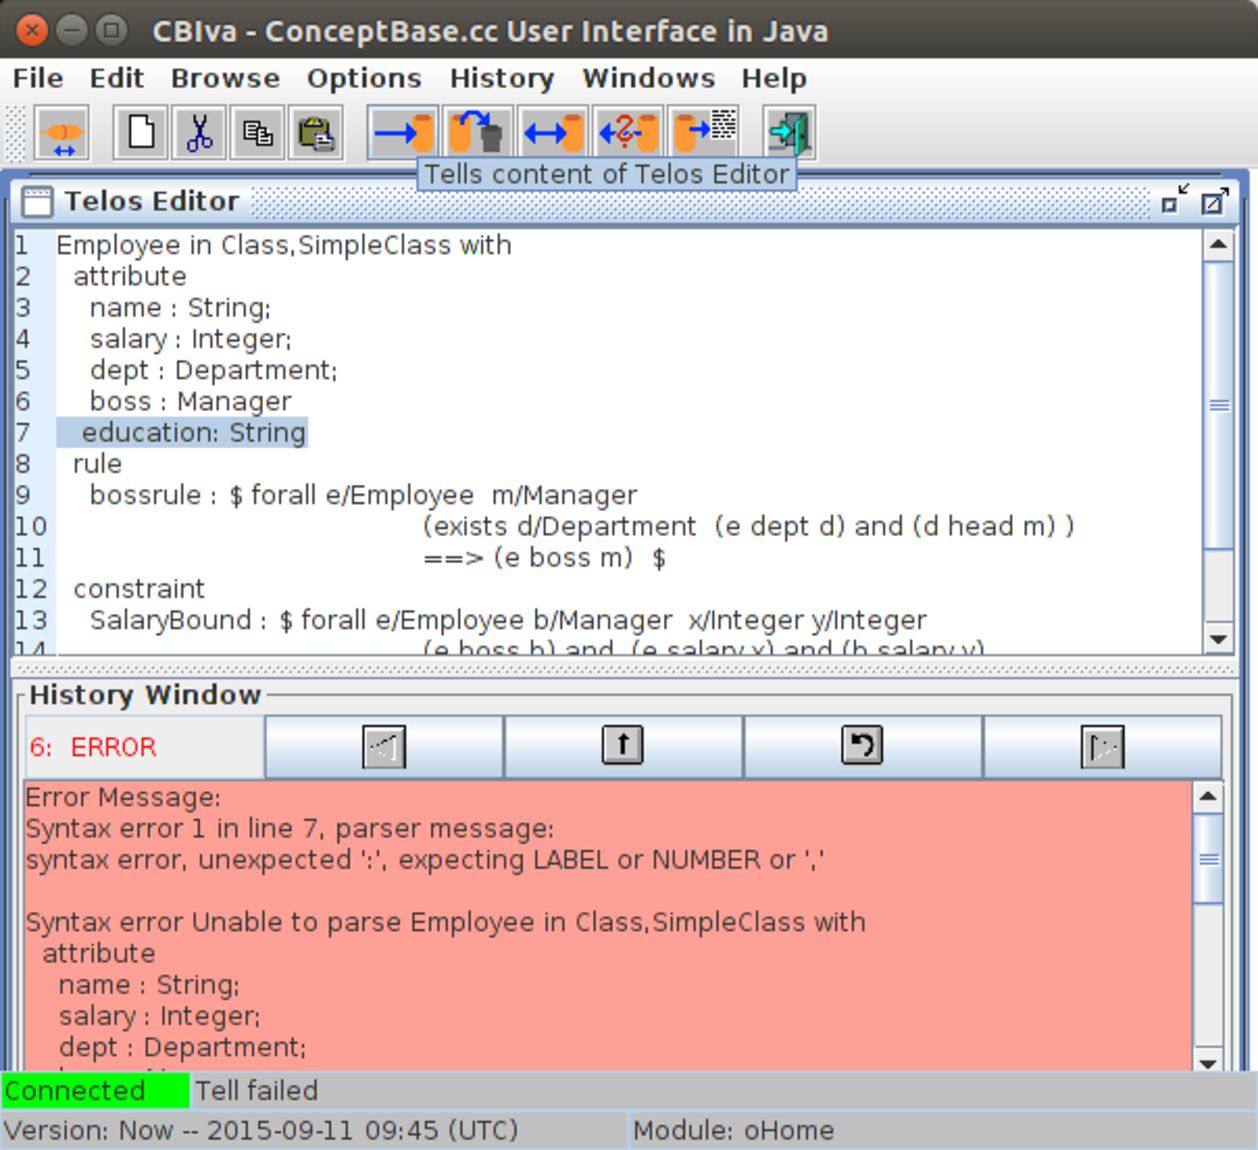
\includegraphics{telos_ed_error.eps}}
              \caption{\label{fig:Telos_ed_error} Trying to add an attribute to the class {\tt Employee} with the 
resulting error report. }
\end{figure}



\subsection{Storing Objects to External Files}


It is possible to store all instances of a class into Unix files by calling 
the menu item {\bf Store Frames} from the {\bf Model} submenu in the {\bf Server} menu. Choosing {\tt Employee} as 
classname, {\tt Employee\-\_Instances} as output-filename and the home directory 
as absolute path will produce a file {\tt Employee\-\_Instances.sml} with all the 
instances of {\tt Employee} in frame representation. If this file already exists 
one is asked to determine whether the program should append the models to 
the file or overwrite it. Note that the extension `{\tt .sml}' is automatically 
added to the end of the filename, so that the menu item {\bf Load Model} will recognise the file as a Telos model-file.




\subsection{Using the Query Facility}


We now want to ask the server for all {\tt Employees} working for {\tt Angus}. We 
first clear the window of the Editor field  by clicking
 the {\bf Clear} menu item. After defining a   new query object 
({\tt AngusEmployees}) (see Figure \ref{fig:query_answer}) we select the {\bf Ask} menu item. 
 The query object is then communicated to the {\em ConceptBase} Server, where it will be stored temporarily and evaluated. {\tt AngusEmployees} will not persist in the Knowledge Base - if you'd like to store the QueryClass, you'd have to {\bf Tell} it explicitly. 
The answer is displayed in the Telos Editor field as well as the Protocol field of the {\em ConceptBase\/Workbench} \ . 
 Figure \ref{fig:query_answer} shows the 
{\em ConceptBase\/Workbench}\ containing the query class and the answer.

\begin{figure}[htb]
              \centering
             \resizebox{13cm}{!}{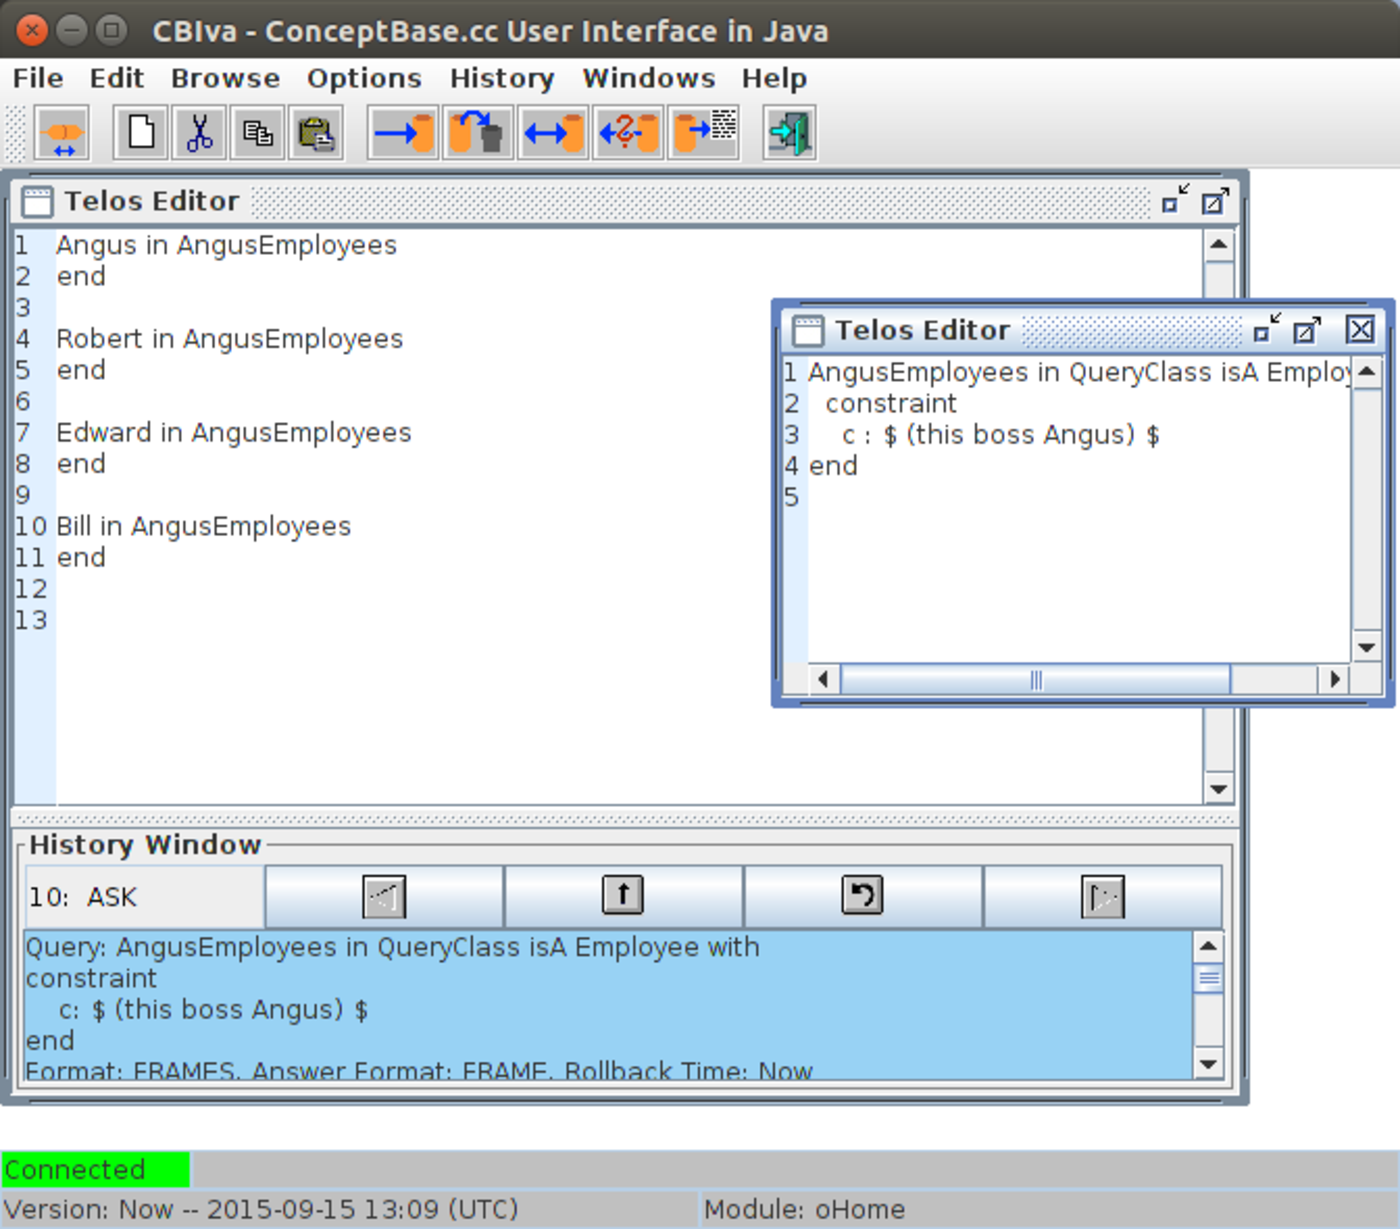
\includegraphics{query_answer.eps}}
              \caption{\label{fig:query_answer}  Query class and its answer. }
\end{figure}

